\documentclass[12pt]{article}
\usepackage{amsmath}
\usepackage{fancyhdr}
\usepackage{hyperref}
\usepackage{graphicx}
\newcommand{\compactlist}{\setlength{\itemsep}{0pt} \setlength{\parskip}{0pt} \setlength{\leftskip}{-1em}}
\usepackage[top=0.9in, bottom=0.8in, left=0.9in, right=0.9in]{geometry}

\lhead{MATH 4263/5373}
\rhead{Nov. 18, 2019}
\chead[RE]{Round-off in numerical differentiation}
\cfoot{}
%\rfoot{Code for figure and report is available in the class folder.}
\pagestyle{fancy}
\begin{document}
Consider the function \(f(x) = e^x\) at a point \(x_0=1\) and approximations to its derivative \(f'(x_0)\approx 2.71281\).  Approximations can be made by to somewhat straightforward approximations: the forward difference and the centered difference.  The error in these approximations is illustrated below, with rounding to simulate calculations by single-precision and double-precision numbers.

\begin{figure}[h!]\centering
\begin{minipage}{0.48\textwidth}
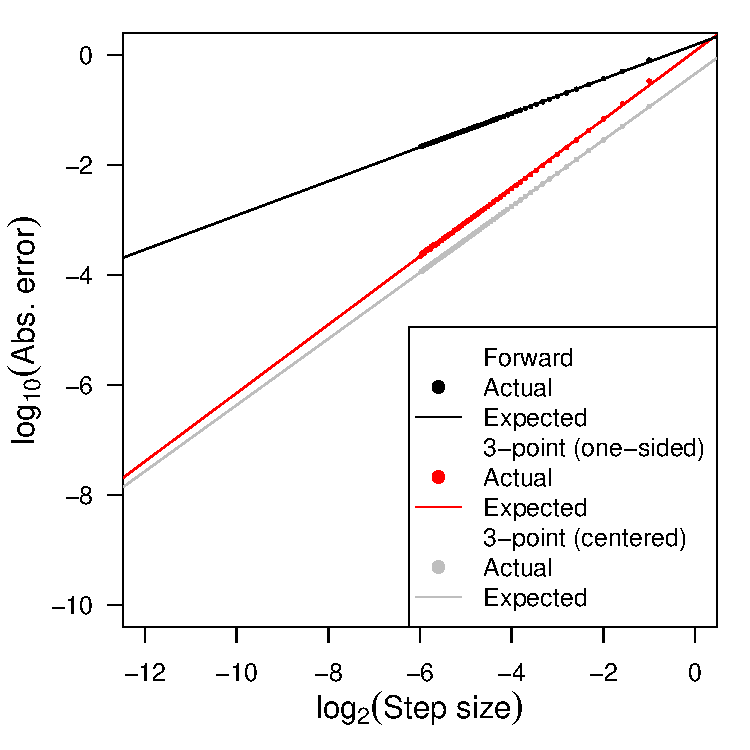
\includegraphics[width=0.9\textwidth]{step_size_8.pdf}

\end{minipage}
\begin{minipage}{0.48\textwidth}
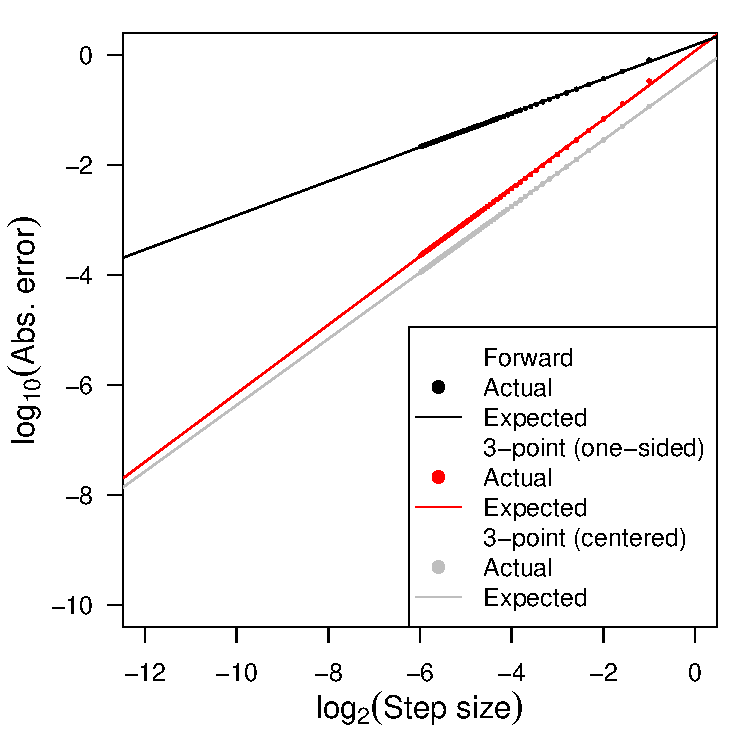
\includegraphics[width=0.9\textwidth]{step_size_16.pdf}

\end{minipage}

\caption{Points indicate calculated \(\log_{10}\left(\text{abs. error}\right)\) for forward (black) and centered (gray) difference approximations.  Line illustrates predicted reduction in error as step size shrinks.  \textbf{Left:} 8 digit calculation (simulated single-precision),  \textbf{Right:} 16 digit calculation (simulated double-precision)}\label{fig::plots}
\end{figure}
%

\begin{figure}[h!]\centering
\begin{minipage}{0.48\textwidth}
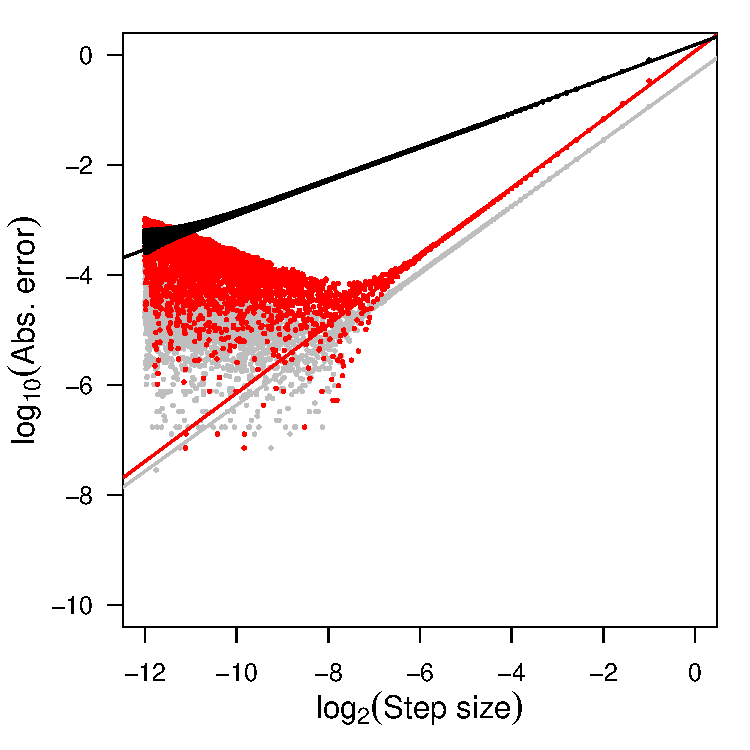
\includegraphics[width=0.9\textwidth]{step_size_roundoff_8.pdf}

\end{minipage}
\begin{minipage}{0.48\textwidth}
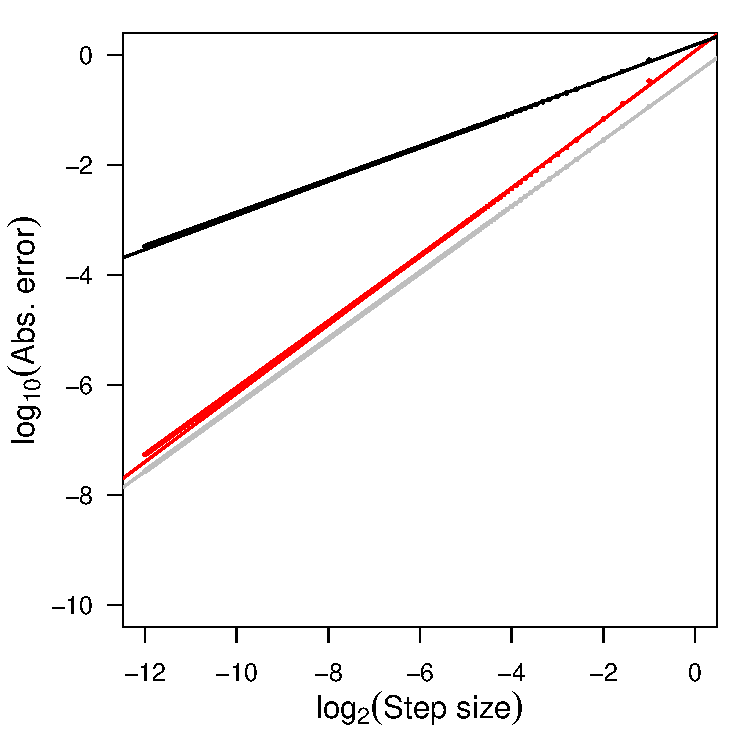
\includegraphics[width=0.9\textwidth]{step_size_roundoff_16.pdf}

\end{minipage}

\caption{As in Figure~\ref{fig::plots}, but with smaller step sizes included.  Note that error \textit{increases} due to roundoff for both methods, but especially for the centered method as the step size is reduced below \(h = 0.01\).}\label{fig::roundoff}
\end{figure}
%

%
%\begin{table}[h!]\centering
%\begin{tabular}{cc}
%\hline
%\(r\) & Sample shape or example\\
%\hline\hline
%\(0<r<1\) & square root function (\(r=0.5\))\\
%\(r=1\) & linear function \\
%\(r>1\) & quadratic or cubic functions
%\end{tabular}
%\end{table}

\end{document}